\chapter{Propuesta Pedagógica}

En este capítulo pasamos a detallar la ventaja pedagógica que se pretende obtener en en base a los objetivos que presentamos en el segundo capítulo y a los antecedentes vistos en el tercero.



\section{Análisis de las soluciones}

% Primero tendrías que decir que la solución a todos los males comentados es tener una forma de integración continua y por qué, después decir qué alternativas hay

Nos gustaría proponer una metodología donde los alumnos usen herramientas que van a tener que usar en futuro profesional (o académico) como pueden ser los sistemas de control de versiones y los sistemas de integración continua, o \textit{continuous integration (CI)}, hay que tener en cuenta que esta metodología está enfocada mayoritariamente a la Formación Profesional porque es la que más asignaturas relacionadas con la programación, como veremos mas adelante. Como la finalidad Formación Profesional es enseñar una profesión enseñarles a nuestros alumnos a usar estos sistemas les va a ser de gran ayuda a la hora de conseguir empleo.

\bigskip
Las tres soluciones libres descritas en los antecedentes (Coderunner, Python Tutor y Jupyter Notebooks) obligan a nuestros alumnos a aprender a usar una herramienta concreta que posiblemente no vayan a volver a utilizar jamás. Esto sería comparable a lo que didácticamente decimos de que el alumno ``aprende a aprobar exámenes'' mas que aprender los contenidos de la asignatura.

\bigskip
Por eso hemos optado por utilizar dos de las tecnologías más utilizadas para gestión de código fuente e integración continua como pueden ser GitHub y Travis CI. Además, ambas son de uso gratuito para proyectos de software libre, fomentando así su uso como se indica en la Orden de 21 de febrero de 2005, sobre disponibilidad pública de los programas informáticos de la Administración de la Junta de Andalucía y de sus Organismos Autónomos.

\section {Temario relacionado con la programación informática}

Tal y como indica el Decreto 110/2016  de 14 de junio, por el que se establece la ordenación y el currículo del Bachillerato en la Comunidad Autónoma de Andalucía las tecnologías de la información y de la comunicación para el aprendizaje y el conocimiento se utilizarán de manera habitual como herramientas integradas para el desarrollo del currículo. Asimismo en los currículos de las distintas ramas educativos donde podemos ejercer como profesores incluyen asignaturas relacionadas con la informática y de forma más específica con la programación informática.


\bigskip
Tecnologías de la Información y Comunicación es un término amplio que enfatiza la integración de la informática y las telecomunicaciones, y de sus componentes hardware y software, con el objetivo de garantizar a los usuarios el acceso, almacenamiento, transmisión y manipulación de información. Su adopción y generalización han provocado profundos cambios en todos los ámbitos de nuestra vida, incluyendo la educación, la sanidad, la democracia, la cultura y la economía, posibilitando la transformación de la Sociedad Industrial en la Sociedad del Conocimiento.

\bigskip
La oferta de asignaturas de informática es variopinta, pues en la Educación Secundaria y Bachillerato es muy básica pero muy específica en la Formación Profesional, por lo que es complejo tener una metodología que se adapte a todos los niveles. Asimismo, los temarios suelen ser bastante extensos incluyendo tanto contenido que es muy difícil abordar cada tema en profundidad. Aquí podemos ver una de las ventajas de nuestra propuesta ya que por un lado, el tiempo que ahorramos lo podemos invertir en impartir más contenidos y que podemos centrarnos en las partes donde fallan los alumnos al ver el histórico de sus errores.

\bigskip
A continuación vamos a enumerar las distintas asignaturas relacionadas con la informática que se pueden encontrar en los currículos de Educación Secundaria, Bachillerato y Formación Profesional, además indicaremos cuales son candidatos a utilizar nuestra metodología en base a sus contenidos.

\subsection {Educación Secundaria Obligatoria (ESO)}

En la Orden de 14 de julio de 2016 se especifica el currículo de la materia de ``Tecnologías de la Información y Comunicación'' que es una materia de opción del bloque de asignaturas específicas para el alumnado de cuarto curso de la Educación Secundaria Obligatoria. Es una asignatura de carácter optativo que intenta dar una visión global de la informática, con lo que su temario intenta abarcar desde historia de la informática hasta la seguridad o la programación web pasando por la ofimática y estudio de los elementos de hardware, nuestra metodología propuesta podría servir de ayuda para la enseñanza de programación de páginas web con HTML que es uno de los contenidos que se dan en dicha asignatura.

\subsection {Bachillerato}

En la Orden de 14 de julio de 2016, por la que se desarrolla el currículo correspondiente al Bachillerato en la Comunidad Autónoma de Andalucía indica las diferentes modalidades de bachillerato, incluyendo las modalidades de Ciencias y la de Humanidades y Ciencias Sociales las asignaturas de carácter obligatorio ``Tecnologías de la Información y de la Comunicación I'' y ``Tecnologías de la Información y de la Comunicación II'' y habiendo también una asignatura de libre configuración autonómica llamada ``Programación y Computación''. Estas asignaturas contienen contenidos de programación informática y de programación de páginas web por lo tanto son susceptibles de utilizar nuestra metodología de realización de ejercicios.

\subsection {Ciclo Formativo Grado Medio}

La Orden EDU/2187/2009, de. 3 de Julio establece el currículo del ciclo formativo de Grado Medio correspondiente al título de ``Técnico en Sistemas Microinformáticos y Redes (SMR)'' que es el único ciclo de grado medio relacionado con la informática donde la única asignatura ligeramente relacionada con la programación es ``Aplicaciones web'', pero dicha asignatura se centra más en el despliegue de aplicaciones que en la programación en sí, por lo que aunque nuestra metodología se podría adaptar para enseñar a configurar como desplegar aplicaciones web no entra dentro del alcance de este trabajo por lo que se deja como posible trabajo futuro.

\subsection {Ciclo Formativo Grado Superior}

Existen tres ciclos formativos de grado superior del plan LOE relacionados con la informática, la Orden EDU/392/2010, de 20 de enero, por la que se establece el currículo del ciclo formativo de Grado Superior correspondiente al título de ``Técnico Superior en Administración de Sistemas Informáticos en Red'' describe las asignaturas ``Lenguajes de Marca y Sistemas de Gestión de Información'' y ``Gestión de Bases de Datos'' en las que nuestra metodología se puede aplicar para corregir los ejercicios ya que se enseñan los lenguajes HTML, SQL, Javascript, XML así como algunos subconjuntos de XML como son DTD y XSD. Los currículos del título de ``Técnico Superior en Desarrollo de Aplicaciones Web'' definido en la Orden EDU/2887/2010, de 2 de noviembre y el de ``Técnico Superior en Desarrollo de Aplicaciones Multiplataforma'' definido en la Orden EDU/2000/2010, de 13 de julio definen varias asignaturas, algunas comunes, como pueden ser ``Programación'', ``Bases de Datos'' y ``Lenguajes de marcas y sistemas de gestión de información'' y otras específicas de cada título como pueden ser ``Programación multimedia y dispositivos móviles'' o ``Desarrollo web en entorno cliente'' que están centradas en el aprendizaje de la programación informática y en los que si encajaría nuestra metodología.

\subsection {Formación Profesional Básica}

La Orden ECD/1030/2014, de 11 de junio define el ``Título Profesional Básico en Informática y Comunicaciones'' y la Orden ECD/1633/2014, de 11 de septiembre define el  ``Título Profesional Básico en Informática de Oficina'', siendo ambas titulaciones las únicas relacionadas con la informática de todas las que componen la formación profesional básica, pero al igual que con el ciclo formativo de Grado Medio ambos currículos carecen de temario específico de programación por lo que queda fuera del ámbito de este proyecto.


% Sería interesante que después de esto destacases la complejidad de tener una metodología de trabajo que permita cubrir los diferentes niveles de complejidad y conceptos que los estudiantes deben aprender, y cómo afrontas ese reto. También puedes decir que la mayoría de temarios (especialmente el de bachillerato) están muy sobrecargados de contenidos lo que resta tiempo para hacer mucha variedad de ejercicios en clase, lo que apoya tu propuesta... En definitiva, que saques de toda esta descripción cosas en claro que apoyen tu visión


\section{Encuesta de percepción}

Se realizó una breve encuesta y se difundió entre algunos profesores de diferentes ámbitos con el fin de ver si nuestra hipótesis de que la corrección de ejercicios era la tarea más tediosa que realizaban como docentes.

\bigskip
Aprovechamos la encuesta para obtener también algunos datos interesantes sobre la forma de trabajar de los docentes, de cara a trabajos futuros. La encuesta se podía consultar en la siguiente dirección web: \url{https://forms.gle/xxSz6mQDjswo5B137}.

\bigskip
La encuesta estuvo activa desde el 19 hasta el 25 de Mayo de 2019 y se recopilaron un total de 47 respuestas. Es una población pequeña pero aun así es interesante por las características de la misma ya que la encuesta se compartió ``de boca a oreja'' indicando que sólo lo compartieran con otros profesores a ser posible relacionados con la informática para no desvirtuar las respuestas.


\begin{enumerate}

\item \textbf{¿Dónde sueles impartir tus clases?}

Con esta pregunta queríamos tener una visión de la población encuestada, ya que al difundirla entre profesores y animarles a compartirla entre sus compañeros profesores era muy posible que sus red de contactos no se limitara a profesores de Educación Secundaria, así que dejamos elegir entre las siguientes opciones:

\begin{itemize}
    \item Educación Primaria
    \item Educación Secundaria
    \item Universidad (Grado/Máster)
    \item Practicas MAES
\end{itemize}

\bigskip
La gran mayoría de los encuestados han resultado ser profesores de Educación Secundaria, por lo que los resultados han sido satisfactorios, los siguientes han sido estudiantes en prácticas en el \master los cuales podríamos englobar dentro del conjunto de los de Secundaria, llegando así casi al 90\% de la población encuestada. Le siguen la respuestas de algunos profesores de Universidad y por último algunos maestros de Educación Primaria.

\begin{figure}[H]
\centering
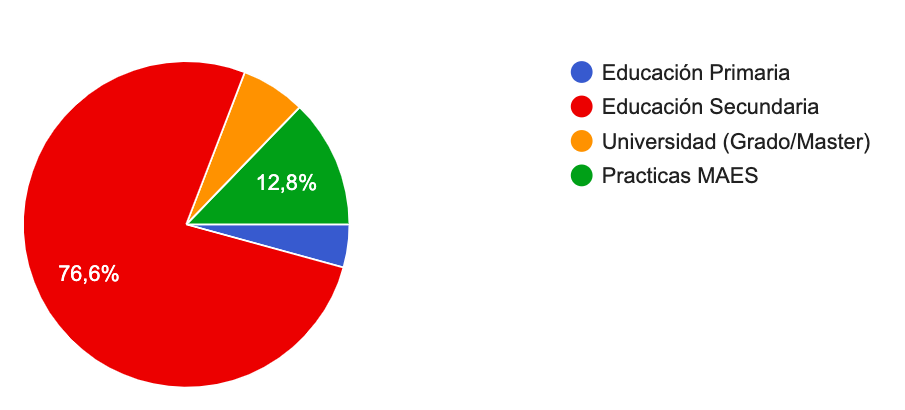
\includegraphics[width=1.0\textwidth]{../images/quiz_1}
\caption{¿Dónde sueles impartir tus clases?}
\label{fig:quiz_1}
\end{figure}


\item \textbf{Valora las siguientes tareas que sueles realizar}

Esta es quizá la pregunta más importante de toda la encuesta, porque queríamos saber la opinión de diversos profesores sobre las tareas de corrección de ejercicios y/o exámenes. Además nos ha servido para hacernos una idea de lo que opinan de las tareas más comunes de un profesor, había que valorarlas según se consideraban ``divertidas'', ``normales'' o ``tediosas'' entendiéndose tediosas como aburridas. Las opciones eran las siguientes:

\begin{itemize}
    \item Preparación de material
    \item Preparación de clases
    \item Impartir clases
    \item Corrección de ejercicios
    \item Evaluación final
    \item Tutorías
\end{itemize}

Como podemos ver, la hipótesis de que corregir ejercicios resulta tedioso ha sido validada. De hecho ha sido la única de las opciones que no ha recibido ningún voto como actividad ``divertida''. Del resto de preguntas podemos deducir que a la mayoría de profesores les divierte impartir clases, esto es algo normal. No tendría sentido una respuesta diferente dado el carácter vocacional de la profesión, y si nos centráramos en los aspectos económicos es mas flagrante en el mundo de la informática porque los sueldos de la empresas privadas están muy por encima de lo que se puede llegar a cobrar como docente. El resto de preguntas se han considerado normales, habiendo opiniones en las tres vertientes. Quizá remarcar que la evaluación es la que menos votos de tarea ``divertida'' han recibido. Aunque esto puede variar mucho de un centro a otro.

\begin{figure}[H]
\centering
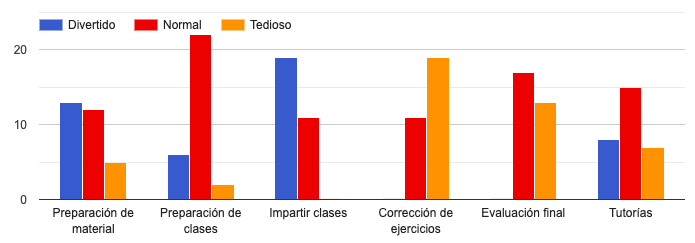
\includegraphics[width=1.0\textwidth]{../images/quiz_2}
\caption{Valora las siguientes tareas que sueles realizar}
\label{fig:quiz_2}
\end{figure}

\item \textbf{¿Elaboras tus propios ejercicios?}

En esta pregunta queríamos saber si los profesores elaboran sus propios ejercicios. En mi experiencia como alumno así como en mi experiencia como docente en prácticas he visto exactamente lo que se ve reflejado en la encuesta, hay profesores que elaboran todo su material, los hay que lo hacen de forma regular pero no siempre, también los hay que los realizan de forma ocasional. Aquí me gustaría remarcar que la opción ``Nunca'' ha recibido muy pocos votos cuando en mi experiencia también hay docentes que utilizan el material de otros profesores en lugar del suyo propio.

\begin{figure}[H]
\centering
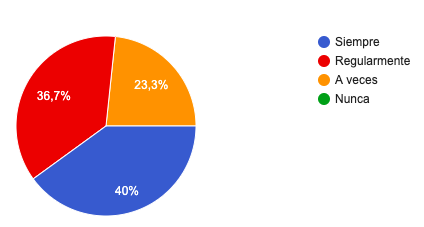
\includegraphics[width=1.0\textwidth]{../images/quiz_3}
\caption{¿Elaboras tus propios ejercicios?}
\label{fig:quiz_3}
\end{figure}

\item \textbf{¿Crees que hay que compartir los ejercicios con el resto de la comunidad?}

Esta pregunta era para ver la repercusión que tiene a nivel docente los conceptos del software libre y las licencias abiertas como la GPL y la ``Creative Commons'' \cite{comons_creative_2013} así como la WikiPedia y otros proyectos que abogan por la difusión libre y gratuita tanto de software como de todo tipo de contenidos culturales.

\bigskip
Por nuestra experiencia pensábamos que no iba a haber tan buena acogida del ``Sí'' como ha habido, pero nos ha sorprendido gratamente que la gran mayoría de los profesores encuestados apoyen el compartir el material. También es algo que se puede considerar normal ya que hoy en día es difícil hacer uso de recursos de terceros encontrados online para apoyar nuestras clases. De hecho en mi periodo como docente en prácticas me sirvió para ver que al contrario que en mi época de estudiante, donde usábamos el libro de texto, los docentes usan recursos como Kahoot!\footnote{Plataforma gratuita que permite la creación de cuestionarios de evaluación en forma de concurso.} o YouTube para hacer las clases mucho mas dinámicas.

\begin{figure}[H]
\centering
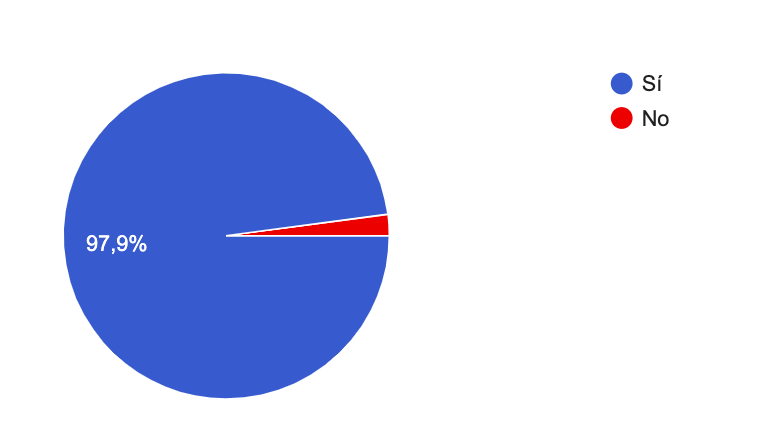
\includegraphics[width=1.0\textwidth]{../images/quiz_4}
\caption{¿Crees que hay que compartir los ejercicios con el resto de la comunidad?}
\label{fig:quiz_4}
\end{figure}

\item \textbf{¿Sueles entregar correcciones de los ejercicios?}

Esta pregunta está íntimamente relacionada con el propósito de este trabajo, queríamos saber si los profesores solían entregar los ejercicios corregidos, hay que tener en cuenta que para que dicha corrección tenga utilidad las correcciones se han de entregar de forma temprana, ya que es cuando el alumno aun está adquiriendo los conocimientos, de dieron las opciones ``Sí'', ``No'' y ``Otra'', siendo esta última opción para que los profesores indicaran alguna opción distinta, a continuación se pega en bruto dichas opciones alternativas:

\begin{itemize}
    \item Algunas veces
    \item A veces y otras se corrigen en clase.
    \item Sí o se corrigen en clase.
\end{itemize}

Nos pareció interesante la opción de la corrección en clase, pues no la habíamos tenido en cuenta, pensamos que es una forma muy didáctica de que el alumno vea dónde ha fallado y hacer una corrección temprana, pero teniendo en cuenta que por norma general siempre hay una sensación de falta de tiempo para impartir el temario, así que quizá invertir tiempo en esta corrección puede hacer que lo perdamos para impartir nuevos contenidos.

\begin{figure}[H]
\centering
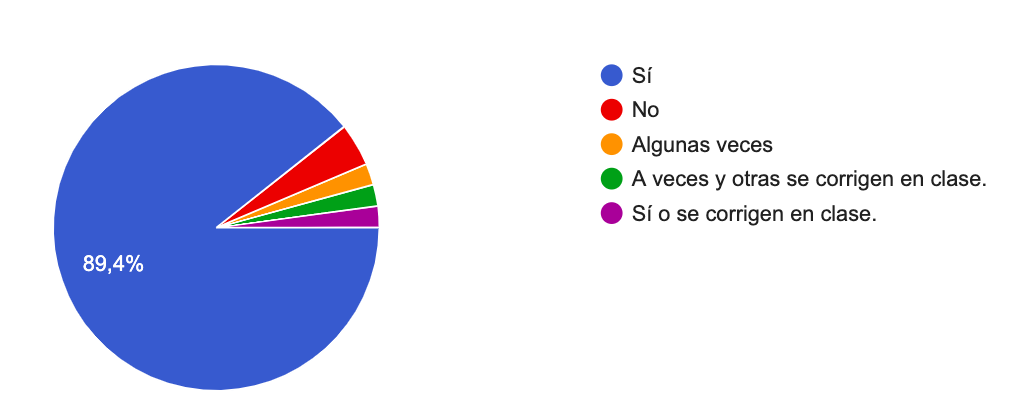
\includegraphics[width=1.0\textwidth]{../images/quiz_5}
\caption{¿Sueles entregar correcciones de los ejercicios?}
\label{fig:quiz_5}
\end{figure}

\item \textbf{¿Qué opinas de los sistemas de corrección automática?}

Aquí preguntamos de forma directa sobre los sistemas de corrección automática de forma genérica, sin especificar ninguno, ya que como hemos visto en los antecedentes existen diversos métodos, aquí les dimos a elegir entre estas opciones:

\begin{itemize}
    \item Ahorran tiempo a alumnos y profesores
    \item Mejoran la enseñanza al poder ver de manera más inmediata los resultados
    \item Desvirtúan la finalidad de los ejercicios propuestos
    \item Deshumaniza la relación profesor-alumno
    \item Otra (especificar)
\end{itemize}

La opción ``Mejoran la enseñanza al poder ver de manera más inmediata los resultados'' fue marcada por casi el 50\% de los encuestados, seguida por la de ``Ahorran tiempo a alumnos y profesores'' que consiguió algo mas del 20\%, ambas en conjunto eran las opciones que eran más acordes al desarrollo de nuestra metodología por lo que podemos ver que hay un claro interés en estos sistemas, además pusimos la opción ``Otra'' donde los profesores indicaron opiniones adicionales que pasamos a enumerar:

\begin{itemize}
    \item Ahorran tiempo a todos y mejoran la enseñanza. Se pueden hacer más ejercicios y practicar mucho es esencial en enseñanzas técnicas.
    \item Sirven para ver si los alumnos han adquirido los conocimientos.
    \item Es otro tipo de herramienta de evaluación.
    \item No lo he probado.
    \item Son útiles en su justa medida.
\end{itemize}

En estas respuestas vemos que en su mayoría también coinciden que los sistemas de corrección automática son muy útiles para mejorar la enseñanza, así que creemos que esta propuesta metodológica puede ser de gran ayuda a profesores.

\begin{figure}[H]
\centering
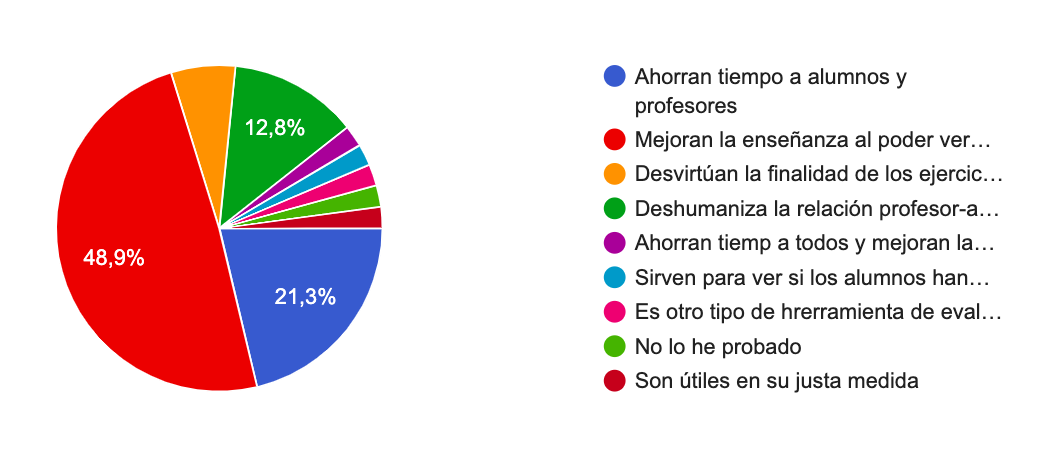
\includegraphics[width=1.0\textwidth]{../images/quiz_6}
\caption{¿Qué opinas de los sistemas de corrección automática?}
\label{fig:quiz_6}
\end{figure}

\item \textbf{Sugerencias para mejorar las clases}

Incorporamos a la encuesta un apartado para que los profesores aportaran sus sugerencias para mejorar las clases, a continuación vamos a poner los datos recopilados en bruto en dicho apartado:

\begin{itemize}
    \item Hacerlas dinámicas y participativas, huir de la explicación meramente.
    \item Lo más eficiente para el aprendizaje del alumnado es que ellos mismos corrijan, así si se les indican los errores suelen verlos y evitarlos después.
    \item Que parte de la evaluación la hagan los propios alumnos (son más conscientes de los errores cometidos).
    \item Fomentar el trabajo basado en proyectos colaborativos.
    \item Correcciones en clase de la totalidad de los ejercicios, haciendo partícipes a los alumnos.
    \item Coevaluación, aula invertida. Cooperativo.
    \item Participación continuada de alumno.
    \item La tipología de ejercicio más eficiente a la hora de su corrección es el tipo test. Existe una optimización de tiempo de corrección bastante notable en comparación con ejercicios con preguntas de desarrollo, donde se tarda más por no tener tan automatizada la respuesta correcta (hay que leer la respuesta), la puntuación se somete a matices por estar incompleta, en ocasiones es difícil comprender la letra del alumno, etc.
\end{itemize}


\end{enumerate}

\section{Definición de la metodología}

% ok con que contrastas con el test, pero me falta lo que te comentaba antes que metieses en otras secciones: una discusión acerca de la naturaleza de los ejercicios, por qué es útil emplear una solución como la tuya, etc.

Tras validar que nuestra propuesta efectivamente tiene un alto valor pedagógico y que encaja dentro de los contenidos de varias asignaturas de los currículos de educación secundaria pasamos a definir los objetivos, contenidos y competencias de nuestra metodología.

\bigskip
El objetivo de nuestra metodología es enseñar programación de una forma diferente, con ejercicios, autocorrección y con tecnologías que se usan en el día a día de cualquier informático que se dedique profesionalmente a ello. La misma nos brinda muchas ventajas como puede ser ver un histórico de los envíos de un alumno, para saber donde falla o el tiempo que le ha dedicado a un ejercicio concreto, un simple vistazo al ``Travis CI'' de cada alumno nos da mucha información, y el poder seguir la traza es muy útil, también podemos ver el historial de \textit{commits} de \textit{Git} de forma rápida para ver la evolución del alumno. El código de colores de \textit{Travis CI} también hace que corregir sea intuitivo, verde para correcto y rojo para incorrecto. En un momento dado podríamos detectar un posible plagio entre alumnos de forma rápida usando el mencionado historial.

\bigskip
Como indica el Decreto 110/2016  de 14 de junio el alumno debe ``conocer el funcionamiento de las nuevas tecnologías de la información y la comunicación, comprendiendo sus fundamentos y utilizándolas para el tratamiento de la información (buscar, almacenar, organizar, manipular, recuperar, presentar, publicar y compartir), así como para la elaboración de programas que resuelvan problemas tecnológicos'' (\cite{junta_de_andalucia_decreto_2016}), así que además de todo lo indicado anteriormente estamos ajustándonos a la normativa.

\bigskip
El decreto anteriormente citado dice que ``la oferta curricular diseñada en este Decreto potencia el desarrollo de las tecnologías de la información y la comunicación, así como la enseñanza de las lenguas extranjeras, teniendo en cuenta los objetivos emanados de la Unión Europea en esta materia y los planes estratégicos de la Comunidad Autónoma de Andalucía para el desarrollo de las lenguas'' por lo que todos los ejercicios propuestos han sido realizados en inglés ya que es el idioma predominante en la informática y nuestros alumnos deberán adquirir competencias de lectura y comprensión en lengua inglesa para poder aprender por si mismos, de hecho el comando \textit{Git} y las páginas \textit{GitHub}, \textit{Travis CI} están completamente en inglés así como la mayor parte de la documentación de lenguajes de programación. Sin ir mas lejos la propia programación informática define sus directivas en inglés, con palabras como ``function'', ``class'' ``for'', ``if'', ``then'' o ``while''.

\subsection{Contenidos}

Los contenidos de nuestra metodología comprenderán dos partes. Una parte común a todas las asignaturas donde se enseñará a usar Git y algunos conceptos básicos de programación y otra específica donde haciendo uso de lo aprendido en la parte común se seguirá el temario de la asignatura en cuestión.

% Eso de que la introducción a la programación se pueda poner o quitar es muy relativo, explícalo mejor

\bigskip
La parte común comprenderá los siguientes dos apartados que se definirán de modo mas extenso en la propuesta metodológica:

\begin{itemize}
    \item Aprendiendo a usar Git: Comandos básicos, creación de una cuenta en GitHub, integración continua, realizar un \textit{fork} del repositorio de ejercicios ...
    \item Introducción a la programación: Conceptos comunes a todos los lenguajes como ``variable'' y ``constante'', condicionales y bucles,...
\end{itemize}

Esta parte común podrá resumirse o incluso obviarse si los alumnos ya conocen alguno de los dos conceptos básicos por haberlos aprendido en otra asignatura.

\bigskip
La parte específica se desarrollará en base a los contenidos de la asignatura a impartir, pero en la propuesta metodológica se definirán algunos ejercicios de ejemplo de diferentes asignaturas como pueden ser ``Lenguajes de marcas y sistemas de gestión de información'', ``Programación'' o ``Bases de Datos''.

\bigskip
Los ejercicios de la parte específica estarán siempre disponibles en su totalidad para que los alumnos puedan ir avanzando al ritmo que deseen. Cada ejercicio tendrá una breve explicación de lo que se requiere y una serie de test TDD que deberán pasar. El profesor también podrá poner ejercicios resueltos pero con algunos errores para que los alumnos los corrijan.

\subsection{Competencias}

La programación informática, y por extensión nuestra metodología, permite adquirir las siguientes 5 del total de 7 competencias clave de la LOMCE descritas en la Orden ECD/65/2015, de 21 de enero:

\begin{itemize}
    \item \textbf{CCL}: Competencia en comunicación lingüística
    \item \textbf{CMCT}: Competencia matemática y competencias básicas en ciencia y tecnología
    \item \textbf{CD}: Competencia Digital
    \item \textbf{CPAA}: Competencia de aprender a aprender
    \item \textbf{SIE}: Sentido de la iniciativa y espíritu emprendedor
\end{itemize}

Entrando en detalle, de nuestra metodología, podemos destacar y definir las siguientes tres:

\begin{itemize}

    \item Utilizar las tecnologías de la información y la comunicación de modo habitual en el proceso de aprendizaje, buscando, analizando y seleccionando información relevante en Internet o en otras fuentes,  elaborando documentos propios, haciendo exposiciones y argumentaciones de los mismos y compartiendo éstos en entornos apropiados para facilitar la interacción.

    \item Conocer el funcionamiento de las nuevas tecnologías de la información y la comunicación, comprendiendo sus fundamentos y utilizándolas para el tratamiento de la información (buscar, almacenar, organizar, manipular, recuperar, presentar, publicar y compartir), así como para la elaboración de programas que resuelvan problemas tecnológicos.

    \item Asumir de forma crítica y activa el avance y la aparición de nuevas tecnologías, incorporándolas al quehacer cotidiano.

\end{itemize}

\subsection{Proceso de entrega}
Para la entrega de ejercicios el alumno deberá realizar un ``Pull request'' contra el repositorio del profesor lo cual dará el ejercicio por entregado. El repositorio tiene una plantilla para la creación de dichos \textit{pull requests} en la que al alumno comprobará un checklist indicando que ha leído el guión de la práctica, cumple los posible pre-requisitos (por ejemplo haber terminado un ejercicio previo) así como indicar que el código entregado es original y no ha tratado de hacer modificaciones en el TDD ni en el \textit{pipeline} (figura \ref{fig:github_pr_create}).

\begin{figure}[h!]
\centering
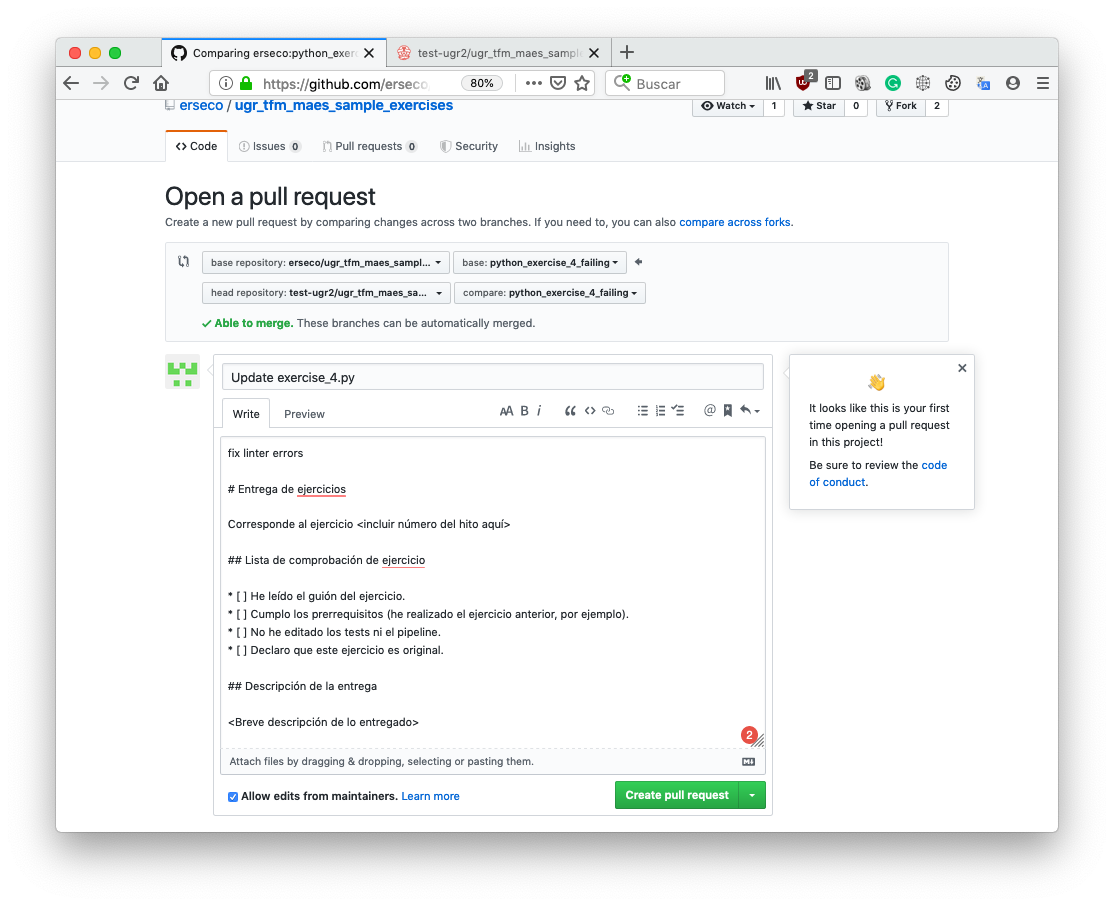
\includegraphics[width=1.0\textwidth]{../images/github_pr_create}
\caption{Plantilla de creación de Pull Request}
\label{fig:github_pr_create}
\end{figure}

Al crear el \textit{pull request} el alumno deberá verificar que no hay conflictos con el código base, si los hubiera deberá corregirlos manualmente. Tras esto se lanzarán los \textit{pipelines} del repositorio del alumno (se activan en cada envío) y el del repositorio del profesor, que se activa al crear el \textit{pull request} (figura \ref{fig:github_pr_view}) y al hacer cualquier envío adicional a la rama asociada al \textit{pull request}. Tras terminar el proceso de ejecución del \textit{pipeline} veremos si este ha dado un error (figura \ref{fig:travis_pipeline_failed}) o ha terminado de forma satisfactoria (figura \ref{fig:travis_pipeline_passed}) siendo esta última la imprescindible para proceder a corregir el ejercicio.

\begin{figure}[h!]
\centering
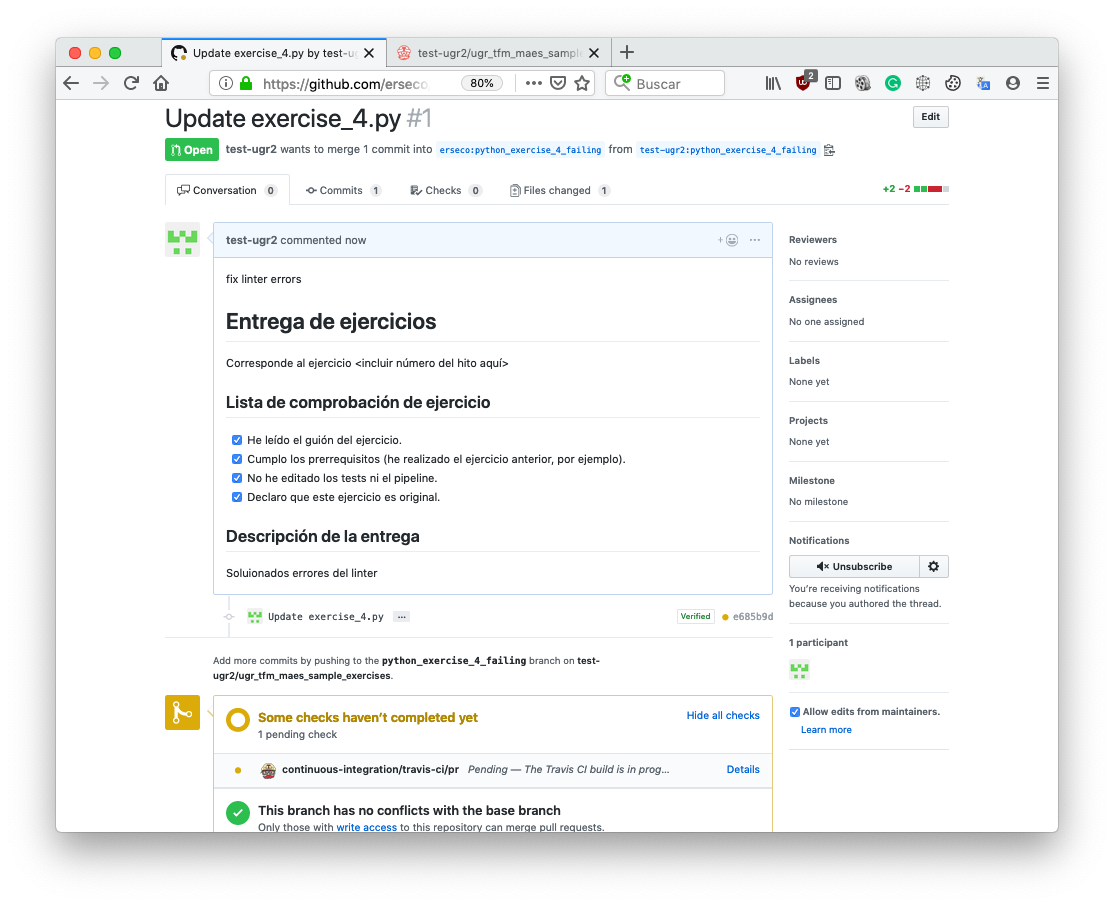
\includegraphics[width=1.0\textwidth]{../images/github_pr_view}
\caption{Vista de un Pull Request creado con el pipeline en ejecución}
\label{fig:github_pr_view}
\end{figure}

\begin{figure}[h!]
\centering
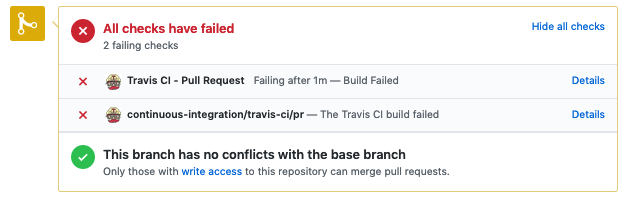
\includegraphics[width=1.0\textwidth]{../images/travis_pipeline_failed}
\caption{Detalle de un pipeline fallido}
\label{fig:travis_pipeline_failed}
\end{figure}

\begin{figure}[h!]
\centering
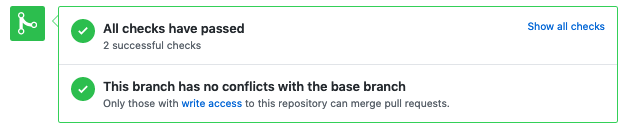
\includegraphics[width=1.0\textwidth]{../images/travis_pipeline_passed}
\caption{Detalle de un pipeline satisfactorio}
\label{fig:travis_pipeline_passed}
\end{figure}

\section{Evaluación}

Para la evaluación de los ejercicios nos basaremos en primer lugar en si han seguido los pasos indicados de forma correcta, realizando un ``Pull request'' e indicando lo realizado, luego comprobaremos si los ``pipelines'' han pasado de forma correcta y de forma adicional podemos entrar a valorar, como hemos mencionado anteriormente, el histórico de envíos a GitHub para ver si ha ido solucionando los problemas de forma adecuada y también valorando el tiempo dedicado. Esto no quiere decir que a mas tiempo mayor calificación, pero si que sirve para hacernos una idea del esfuerzo que ha invertido el alumno para solucionar los ejercicios. Esto no quiere decir que también se pueda realizar una corrección ``manual'' de los ejercicios si fuera necesario.

\bigskip
Una utilidad muy útil de nuestro sistema es que podemos ver los cambios de forma visual con la pagina de diferencias, o \textit{diff} (figura \ref{fig:github_pr_diff}) lo que nos permite centrarnos en los cambios que ha realizado el alumno, además de detectar cualquier posible intento de modificación del código del \textit{pipeline} o de los tests de verificación, con esto nos podemos asegurar en la evaluación de que todo lo entregado por el alumno está realizado conforme al guión entregado.

\begin{figure}[h!]
\centering
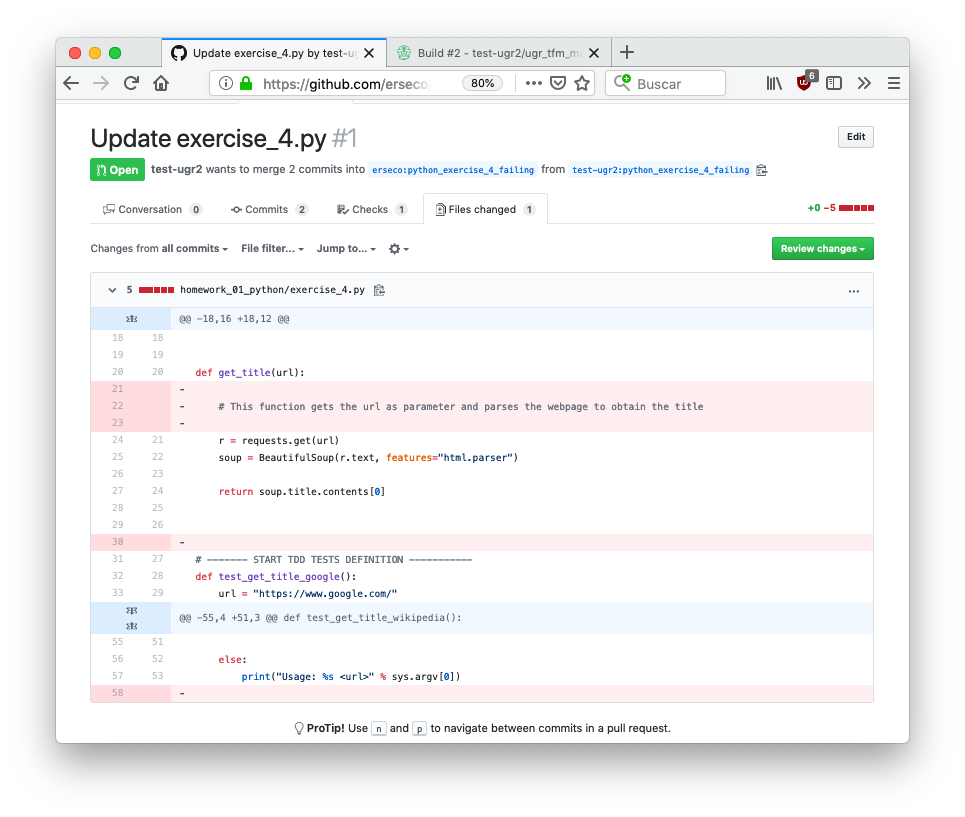
\includegraphics[width=1.0\textwidth]{../images/github_pr_diff}
\caption{Detalle de los cambios de código en un Pull Request}
\label{fig:github_pr_diff}
\end{figure}



% Falta mucho aquí acerca de la forma de trabajar: cómo plantear los ejercicios, cómo hacerlos con distintos objetivos y niveles, cómo se puede plantear la evaluación y calificación.... todo eso es parte de tu propuesta que puede ser un poco "independiente" de la propuesta tecnológica



